\section{Feature Selection}
% TODO: review this section
Feature selection is the process of choosing a subset of the available
input features that are most relevant to the prediction target, and
discarding those that are redundant or uninformative. Using fewer
features reduces the risk of overfitting, makes the model easier to
interpret and, most importantly for this work, reduces the size of the
model and the cost of inference on a constrained device. It also
reduces the number of metrics each node must measure and share with
its neighbours.

% TODO: have to specify how feature correlation and feature
% importance are different
In this section, we combine filter method: Spearman correlations
which measures the correlation between
features prior to training the model and identify weakly related
features to the output label.
Two widely used examples are permutation importance
\cite{altmannPermutationImportanceCorrected2010} and SHapley Additive
exPlanations (SHAP) \cite{lundbergUnifiedApproachInterpreting2017},
both described below.
And permutation importance and SHAP after training on a full feature
set to identify the subset of feature.
Decision tree and LGBMTreeRegressor have embedded feature importance
during the training. However, these are not comparable to each other
as the method used to calculate that differ from model to model.

\subsection{Feature Correlation}
Spearman's rank correlation coefficient by measuring how well the
relationship between the two variables can be
described by a \emph{monotonic} function, that is, whether one
variable consistently increases or consistently decreases as the
other increases, regardless of whether the change is linear. Like
Pearson's coefficient, it ranges from $-1$ to $1$. A value of $1$
means that $Y$ always increases when $X$ increases, $-1$ means that
$Y$ always decreases when $X$ increases, and $0$ means there is no
monotonic trend.

To compute the coefficient, each value is first replaced by its
\emph{rank}, its position when the data are sorted, with tied values
given the average of their ranks. The Spearman coefficient is then
the Pearson coefficient between the ranks:
% TODO: review the equation
\begin{equation}
    \rho_{XY} = r_{R(X)\,R(Y)},
\end{equation}
where $R(X)$ and $R(Y)$ are the ranks of $X$ and $Y$. Because the
ranks of a monotonic relationship always lie on a straight line,
Pearson's coefficient on the ranks reaches $\pm 1$ for any perfectly
monotonic relationship, linear or not. For example, if PDR falls
whenever the parent's drop rate rises, $\rho = -1$ even if PDR falls
slowly at first and then sharply

Figure~\ref{fig:feature_correlation} shows the Spearman correlation
between each pair of the 11 collected features and the PDR. Three
observations stand out. First, the features most strongly related to
PDR all describe the load on the path towards the root: the parent's
drop rate ($\rho = -0.69$), the parent's CPU usage ($-0.67$), the hop
count ($-0.66$) and the parent's traffic rate ($-0.55$). All are
negatively correlated with PDR, as expected, since a node behind a
busier parent or a longer path loses more packets. Second, these
features are also strongly correlated with each other. The three
parent metrics have pairwise correlations between $0.72$ and $0.78$,
and hop count is correlated with them by $0.68$ to $0.77$. They
therefore carry much of the same information, so a model may need
only one or two of them. Third, the neighbour count ($0.04$) and RSSI
($-0.16$) are only weakly correlated with PDR, and the neighbour count
is barely correlated with any other feature.

\begin{fig}[tbh]
    \begin{center}
        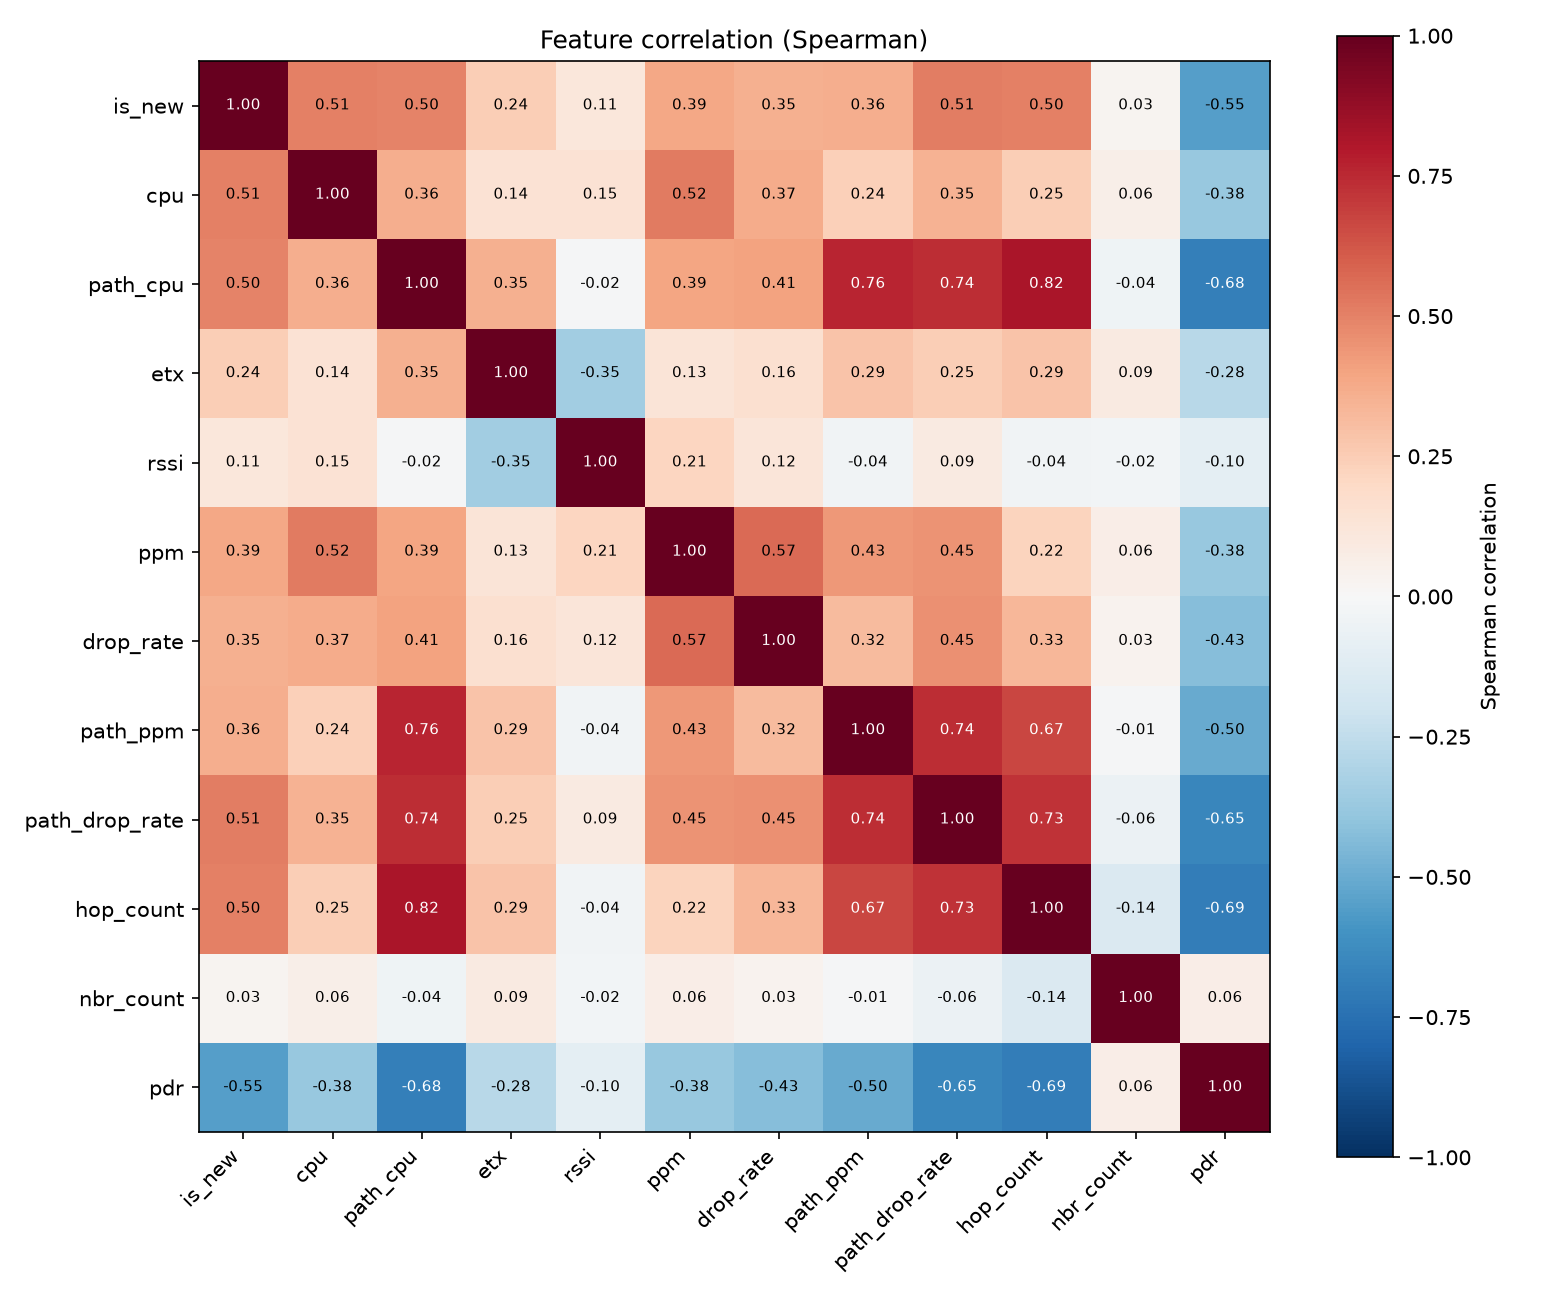
\includegraphics[width=0.9\textwidth]{assets/feature_correlation.png}
        \caption{Spearman feature correlation of 11 collected features.}
        \label{fig:feature_correlation}
    \end{center}
\end{fig}

\subsection{Permutation Importance}
Permutation importance \cite{altmannPermutationImportanceCorrected2010}
inspects how importance each feature is by permutation the value of
each feature in data rows.
The idea is that if a feature is important, breaking its link with
the output should make the model's predictions worse. The method
first measures the model's baseline score $s$ on a dataset. Then, for
each feature $j$, it randomly shuffles that feature's values across
the rows, which keeps the feature's distribution but removes its
relationship with the PDR. The model is scored on this corrupted
dataset, and the shuffle is repeated $K$ times to reduce the effect
of randomness. The importance of feature $j$ is the average drop in
score:
\begin{equation}
    i_j = s - \frac{1}{K} \sum_{k=1}^{K} s_{k,j},
\end{equation}
where $s_{k,j}$ is the score after the $k$-th shuffle of feature $j$.
In this work, the score is the negative mean absolute error, so
$i_j$ is the average increase in prediction error when feature $j$
is shuffled. We use $K = 10$, and compute the importance on a
held-out test set of 20\% of the data, so that it reflects how the
model generalises rather than what it memorised during training.

Permutation importance avoids the main weaknesses of the mean
decrease in impurity (MDI) described above. MDI is calculated from
the training data and favours features with many distinct values,
such as ETX, over low-cardinality features such as the binary
\texttt{is\_new}. Permutation importance does not depend on how the
model splits the data, so it has no such bias, and it can be computed
on unseen data.

However, permutation importance has two limitations. First, it
measures how much the model's \emph{error} depends on a feature does not show
whether a feature pushes the predicted PDR up or down. Second, when
two features are strongly correlated, such as ETX and hop count,
shuffling one of them has little effect because the model can still
rely on the other. Both features may then appear less important than
they really are. Shuffling can also create unrealistic inputs, such
as a node with a high hop count but a very low ETX.

\subsection{SHAP}
SHapley Additive exPlanations (SHAP) is technique that measures the
average magnitude of a feature's contribution to a model's
predictions across a dataset based on cooperative game theory.
Measure how each feature influence the outcome of the model.

Explaining a generalized additive regression model
% TODO: include a bit of math
\cite{lundbergUnifiedApproachInterpreting2017}
\cite{lundbergLocalExplanationsGlobal2020}

We use Tree SHAP is a fast and exact method to estimate SHAP values
for tree models and ensembles of trees

\begin{equation}
    \phi_i = \sum_{S \subseteq F \setminus \{i\}} \frac{|S|!\,(|F| -
    |S| - 1)!}{|F|!} \left[ f_{S \cup \{i\}}\!\left(x_{S \cup
    \{i\}}\right) - f_S\!\left(x_S\right) \right].
\end{equation}
The waterfall model shows the local Interpretability

The Beeswarm works by aggregating local SHAP values from local mode
to see the global trend.

Figure ... shows the feature importance of the model trained on RF
and LGBMTreeRegressor.sd

Afterward, we did train the models on reduce number of features from
1 to 11. From that we choose the ... features, to reduce the size of
the tree significantly while trading the performance of the model minimally.

SHapley Additive exPlanations (SHAP)
\cite{lundbergUnifiedApproachInterpreting2017} is a technique  based
on the Shapley value from cooperative game theory, which divides the
total payout of a game fairly among the players according to each
player's contribution. In SHAP, the ``game'' is a single prediction,
the ``players'' are the input features, and the ``payout'' is the
difference between the model's prediction and its average prediction.
Unlike permutation importance, which measures how much a feature
affects the model's \emph{error}, SHAP measures how much each feature
moves the model's \emph{prediction}, and in which direction.

SHAP explains a prediction with an \emph{additive} model: the
prediction for an input $\mathbf{x}$ is written as a base value plus
one contribution per feature,
\begin{equation}
    f(\mathbf{x}) = \phi_0 + \sum_{i=1}^{M} \phi_i,
\end{equation}
where $M$ is the number of features, $\phi_0 = \mathbb{E}[f(\mathbf{X})]$
is the model's average prediction over the data, and $\phi_i$ is the
SHAP value of feature $i$ for this input. A positive $\phi_i$ means
that feature $i$ raised the predicted PDR above the average, and a
negative $\phi_i$ means it lowered it. Because the contributions add
up exactly to the prediction, each prediction can be broken down into
the share contributed by each feature.

The SHAP value of feature $i$ is its Shapley value: its average
contribution over every possible subset of the other features,
\begin{equation}
    \phi_i = \sum_{S \subseteq F \setminus \{i\}} \frac{|S|!\,(|F| -
    |S| - 1)!}{|F|!} \left[ f_{S \cup \{i\}}\!\left(x_{S \cup
    \{i\}}\right) - f_S\!\left(x_S\right) \right],
\end{equation}
where $F$ is the set of all features, $S$ is a subset of features
that does not include $i$, and $f_S(x_S)$ is the model's expected
prediction when only the features in $S$ are known. The term in
brackets is the change in prediction when feature $i$ is added to
the subset $S$, and the fraction weights each subset so that every
order in which features could be added counts equally. This is the
only attribution method that satisfies a set of fairness properties,
including that the contributions add up to the prediction and that a
feature that never changes the prediction receives a value of zero
\cite{lundbergUnifiedApproachInterpreting2017}.

% TODO: probs don't need this paragraph
Computing this sum directly requires evaluating the model on all
$2^{M}$ subsets of features, which quickly becomes impractical. For
tree-based models, we use Tree SHAP
\cite{lundbergLocalExplanationsGlobal2020}, which exploits the
structure of the trees to compute the exact SHAP values in polynomial
time, $O(TLD^2)$ for an ensemble of $T$ trees with at most $L$ leaves
and depth $D$. It does this by tracking, as it follows every path
through each tree, what fraction of the possible feature subsets
would reach each leaf. This makes it fast enough to explain thousands
of predictions from both the decision tree and LightGBM models.

SHAP values can be viewed at two levels. Locally, a \emph{waterfall
plot} explains a single prediction: it starts from the base value
$\phi_0$ and adds the contribution of each feature in turn, showing
which features pushed the predicted PDR up or down for that node.
Globally, a \emph{beeswarm plot} combines the SHAP values of many
predictions to show the overall trend. Each point is one prediction,
placed horizontally by the feature's SHAP value and coloured by the
feature's value, so the plot shows both how much a feature matters
and whether high or low values of the feature raise or lower the
prediction. To rank the features with a single number, we use the
mean absolute SHAP value of each feature over $n$ predictions,
\begin{equation}
    I_i = \frac{1}{n} \sum_{k=1}^{n} \left| \phi_i^{(k)} \right|,
\end{equation}
which is the average amount by which feature $i$ moves the predicted
PDR. As with permutation importance, we compute the SHAP values on
the held-out test set, using a random sample of 2\,000 rows.
Figure~\ref{fig:shap_beeswarm} shows the beeswarm plots for the
decision tree and LightGBM models, and the mean absolute SHAP values
are listed alongside the permutation importances in
Tables~\ref{tab:fi_dtree} and~\ref{tab:fi_lgbm}.

\subsection{Feature Analysis}
Figure ... shows the correlation and the influence of the features to
the result of the prediction.

From the Table, we remove ETX, RSSI,... out of the features for the model.
Which resulted in reducing ... \% in the performance.

\begin{table}[htbp]
    \centering
    \caption{Feature importance for the decision tree model (MAEP points).}
    \label{tab:fi_dtree}
    \begin{tabular}{l|c|c}
        \hline
        \textbf{Feature} & Permutation & Mean $|\mathrm{SHAP}|$ \\
        \hline
        \texttt{hop\_count}         & 7.402 & 11.319 \\
        \texttt{p\_cpu}             & 7.047 & 15.794 \\
        \texttt{drop\_rate}         & 1.920 &  2.388 \\
        \texttt{parent\_drop\_rate} & 1.242 &  2.827 \\
        \texttt{etx}                & 0.815 &  2.107 \\
        \texttt{is\_new}            & 0.758 &  2.159 \\
        \texttt{rssi}               & 0.635 &  1.328 \\
        \texttt{ppm}                & 0.580 &  1.484 \\
        \texttt{cpu}                & 0.517 &  1.160 \\
        \texttt{parent\_ppm}        & 0.512 &  2.314 \\
        \texttt{nbr\_count}         & 0.099 &  0.434 \\
        \hline
    \end{tabular}
\end{table}

\begin{table}[htbp]
    \centering
    \caption{Feature importance for the LightGBM model (MAEP points).}
    \label{tab:fi_lgbm}
    \begin{tabular}{l|c|c}
        \hline
        \textbf{Feature} & Permutation & Mean $|\mathrm{SHAP}|$ \\
        \hline
        \texttt{p\_cpu}             &  8.661   & 12.868 \\
        \texttt{hop\_count}         &  7.194   & 12.898 \\
        \texttt{parent\_drop\_rate} &  1.465   &  2.569 \\
        \texttt{drop\_rate}         &  1.256   &  1.641 \\
        \texttt{cpu}                &  0.842   &  1.342 \\
        \texttt{ppm}                &  0.776   &  1.472 \\
        \texttt{is\_new}            &  0.716   &  1.595 \\
        \texttt{etx}                &  0.695   &  1.824 \\
        \texttt{rssi}               &  0.234   &  0.808 \\
        \texttt{nbr\_count}         &  0.063   &  0.304 \\
        \texttt{parent\_ppm}        & $-0.037$ &  2.203 \\
        \hline
    \end{tabular}
\end{table}

Afterward, we remove the lowest features subsequent and retrain the
model to obtain new model performance on reduced training features
until the MAEP is larger than 1\% of the best model.

In the end, we removed ... features and keep ... features
The performance of the new model is ..., resulting in ...
This is a reasonable tradeoff between memory, computation and
accuracy for constrained devices
